\documentclass[11pt, class=article, crop=false]{standalone}
\usepackage[subpreambles=true]{standalone}
\usepackage[T1]{fontenc} % for font setting
\usepackage{newtxtext,newtxmath}
\usepackage{import,
            graphicx,
            parskip,
            url,
            amsmath,
            wrapfig,
            fancyhdr,
            soul,
            tabularx,
            authblk}

% side caption figure
\usepackage{sidecap}
\sidecaptionvpos{figure}{t}

% for special characters in bibliography            
\usepackage[utf8]{inputenc}
\usepackage[T1]{fontenc}

% citation setup
\usepackage[euler]{textgreek}
\usepackage[sort&compress]{natbib}
\setcitestyle{square}
\setcitestyle{comma}
\bibliographystyle{bibstyle}

% caption setup
\usepackage[font={f, small}, labelfont={bf, small}]{caption}
           
% color box
\usepackage[most]{tcolorbox}
\tcbuselibrary{breakable}

% margin
\usepackage[top=2.54cm, bottom=2.54cm, left=2.54cm, right=2.54cm]{geometry}%set margin

% title
\title{Geometric ecosystem complexity regulates food chains}
\date{} % remove date from title

% author list
\author[1]{Akira Terui}
\author[1,2]{Shota Shibasaki}
\author[3]{Justin P. F. Pomeranz}
\author[4]{Mason Ibrahim}
\author[5]{Dai Yamazaki}
\author[6]{Jacques C. Finlay}
\affil[1]{Depatment of Biology, University of North Carolina at Greensboro}
\affil[2]{National Institute of Genetics}
\affil[3]{Colorado Mesa University}
\affil[4]{Duke University}
\affil[5]{Institute of Industrial Science, University of Tokyo}
\affil[6]{Departiment of Ecology, Evolution, and Behavior, University of Minnesota}


\begin{document}
\maketitle

\section{Maintext}
Since Charles Elton publicized ``food cycles,'' food webs have been a central theme in ecology.
In particular, the vertical structure of food webs, often measured as food chain length (FCL), has intrigued ecologists due to its implications for trophic dynamics, nutrient cycling, and biomagnification of environmental contaminants.

In theory, FCL should increase with increasing resource availability, environmental stability, and ecosystem size by enhancing the persistence of constituent species.
However, empirical research has reported mixed results for resource availability and environmental stability hypotheses due partly to complex interactions between internal food web structure and environmental drivers.
In contrast, ample evidence suggests that ecosystem size can control FCL in spatially simple ecosystems (e.g., oceanic islands), where the areal extent may capture important ecological processes underlying the ecosystem size hypothesis.
These findings have led to the prevailing view that ecosystem size is a primary regulator of food chains.

Much less appreciated, but potentially important, is the geometric complexity of spatial ecosystem structure (``ecosystem complexity'').
Previous studies on FCL predominantly used simplified landscape models for tractability.
However, many natural systems display intricate structures, characterized by repeating geometric patterns across spatial scales.
For example, branching ecosystems, such as trees and rivers, exhibit deep self-similarity in branching patterns, making this feature characteristic independent of ecosystem size.
The prevalence of branching dictates habitat heterogeneity and connectivity, underpinning the emergent stability of metapopulation dynamics and the spatial coexistence of competing species.
Such influences of ecosystem complexity should ``build up'' in a food web through predator-prey interactions and may regulate food chains.
Yet, scant attention has been paid to ecosystem complexity in food web research, illuminating a critical need for integrating spatial complexity into food chain theory.

Here, we use mathematical theory and meta-analysis to show that ecosystem complexity dictates food chain length in rivers.
Contrary to the prevailing wisdom, our spatial theory predicts indeterminate relationships between FCL and ecosystem size.
Instead, ecosystem complexity, measured as branching rate, emerges as an alternative regulator of FCL, showing consistent positive relationships across various ecological contexts.
Our meta-analysis of global FCL data provides empirical evidence for these theoretical predictions.
The present study offers an important conceptual pillar to understand how food webs are organized in spatially complex ecosystems.

\section{Results and Discussion}

\subsection{Theoretical prediction}

We consider a bifurcating branching ecosystem of total river length $L$ (ecosystem size) and branching rate $\lambda_b$ (ecosystem complexity).
Habitat patches are distributed randomly with density $h$ [river length$^{-1}$] along the river, resulting in the total number of habitat patches $N = Lh$.
In our framework, the branching rate $\lambda_b$ can be viewed as the expected number of links per unit river length, where an individual link (or ``branch'') refers to a river segment from one confluence to another or a terminal point of the river (the upstream origin or the mouth) (Figure XX).
An ecosystem with a higher branching rate may contain more confluences (see \textbf{Methods} for specific assumptions).

We model the patch occupancy dynamics of multi-trophic communities within the branching river network.
Let $p_k$ denote the proportion of habitat patches occupied for species $k$.
We describe the patch occupancy dynamics as:

\begin{equation}
    \frac{dp_k}{dt} = \gamma_{k} p_k (1 - p_k) - \mu_k p_k,
    \label{eq:model0}
\end{equation}

where $\gamma_k$ and $\mu_k$ denote colonization and extinction rates, respectively.
Here, we establish a connection between these parameters and spatial ecosystem properties, i.e., ecosystem size $L$ and complexity $\lambda_b$, as follows.

The colonization rate $\gamma_k$ is the number of effective propagules $c_{0,k}$ that successfully colonize habitat patches with establishment probability $r_k$ ($\gamma_k = c_{0,k} r_k$).
Propagules that survive the dispersal phase are referred to as ``effective''; thus, $c_{0,k}$ is a product of the gross number of propagules produced $g_k$ and survival probability during dispersal $\phi_k$.
However, we impose a habitat constraint on $c_{0,k}$ to realize $N$ is the possible maximum that effective propagules can colonize:

\begin{equation}
    c_{0, k} = 
    \begin{cases}
        g_k \phi_k & \text{if $g_k \phi_k < N$},\\
        N & \text{if $g_k \phi_k \ge N$}.
    \end{cases}
    \label{eq:c0-prod}
\end{equation}

As such, the colonization rate increases with increasing ecosystem size ($N = Lh$) unless being limited by the species' ability to produce effective propagules.
We assumed that the establishment probability is proportional to resource supply $r_0$ for producers or the number of consumable prey for consumers.

The extinction rate comprises three potential sources of extinction, that is, disturbance, prey scarcity, and predation:

\begin{equation}
    \mu_{k} = 
        \underbrace{\mu_{k}^{(0)} (1 + \rho \hat{u})}_{\text{Disturbance}} + 
        \underbrace{\mu_{k}^{(p)} \left(1 - \frac{\sum_{q~\in~\text{prey}} p_{q}}{S_{p, k}} \right)}_{\text{Prey scarcity}} + 
        \underbrace{\mu_{k}^{(c)} \sum_{q~\in~\text{predator}} p_{q}}_{\text{Predation}},
    \label{eq:extn}    
\end{equation}

where $\mu_k^{(0)}$, $\mu_k^{(p)}$, and $\mu_k^{(c)}$ are base parameters scaling the impacts of disturbance, prey scarcity, and predation, $\rho$ is the spatial synchrony probability, $\hat{u}$ is the expected upstream river length from a given habitat patch within a branching network, and $S_{p, k}$ is the number of consumable prey for consumer $k$.
Importantly, this formulation captures the downstream disturbance cascade.
In rivers, any disturbance event occurring upstream can propagate downstream through water movement, such as the spread of chemical contaminants, floods, or droughts.
This propagation can lead to population synchrony across multiple habitats with a certain probability, denoted as the synchrony probability $\rho$. 
We assumed that such a risk of disturbance cascade is proportional to the upstream river length $u$, whose expected value $\hat{u}$ is a complex function of river length $L$ and branching rate $\lambda_b$.
Therefore, the extinction dynamics are also linked to the spatial ecosystem properties.
For simplicity, we assumed constant values across species for $\mu_k^{(0)} \equiv \mu^{(0)}$, $\mu_k^{(p)} \equiv \mu^{(p)}$, and $\mu_k^{(c)} \equiv \mu^{(c)}$.

We evaluated how total river length ($L$) and branching rate ($\lambda_b$) influence food chains across various scenarios characterized by different levels of resource supply ($r_0$) and disturbance regimes ($\mu^{(0)}$).
We employed the preferential prey model to generate XX food webs, each comprising 32 trophic species.
These food webs varied in the number of trophic links and producer species, allowing us to account for potential variations in food web structure.

In the absence of predation effects ($\mu^{(c)} = 0$), the FCL at equilibrium -- defined as the maximum trophic position of persistent species -- can be analytically determined by sequentially solving Equation \ref{eq:model0} for $p_k$ ($dp_k/dt = 0$) from the base to the apex of the food web. 
Contrary to the predictions of the ecosystem size hypothesis, the model indicates that the relationship between FCL and river length ($L$) is either hump-shaped or vague, with a sharp increase only from small to intermediate ecosystem sizes.
In contrast, the branching rate ($\lambda_b$) consistently led to an increase in FCL.
While resource supply positively influenced FCL and disturbance had a negative impact, these factors did not alter the overall qualitative relationships between FCL and ecosystem properties.

\begin{figure}
    \centering
    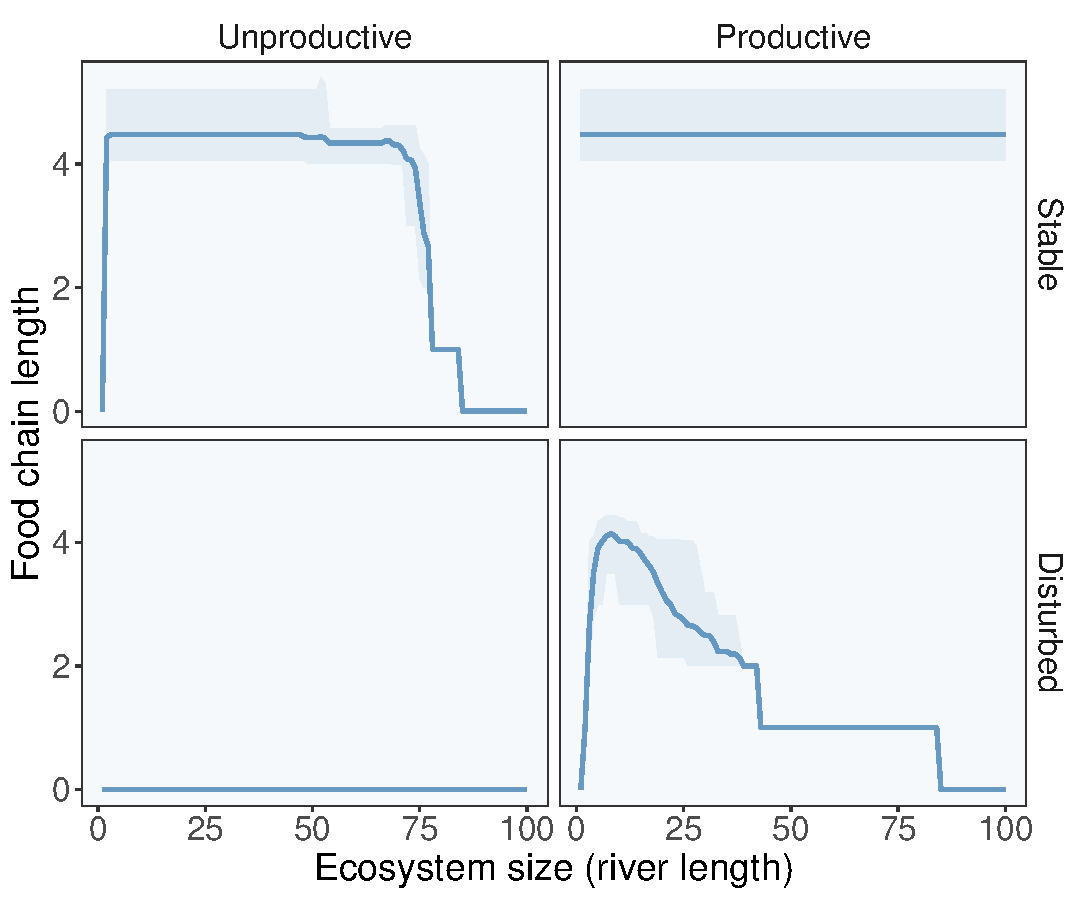
\includegraphics[width=0.5\linewidth]{output/fig_theory_size.pdf}
    \caption{Caption}
    \label{fig:enter-label}
\end{figure}

The analytical predictions remain robust even when relaxing the assumption to include predation effect ($\mu^{(c)} > 0$) and allowing variation in other ecological parameters, such as prey effect ($\mu^{(p)}$), propagule size ($g$), synchrony probability ($\rho$), and trophic omnivory ($\theta$).
In our numerical analysis, the impact of ecosystem size on FCL was highly context-dependent, with FCL increasing with ecosystem size in only a limited number of ecological scenarios.
In contrast, the positive relationship between FCL and branching rate was consistently observed across most ecological scenarios, with only a few exceptions.

The disturbance cascade can explain the counter-intuitive predictions.
In our framework, we assumed that the risk of disturbance cascade increases with increasing upstream river length $\hat{u}$, a monotonic increasing function of total river length $L$ (Figure XX) -- that is, the broader spatial coverage increases the likelihood that an episodic disturbance will occur in some part of the upstream flow-connected area and subsequently cascade downstream.
Consequently, in larger ecosystems, the greater likelihood of synchronized extinctions can offset, or even exceed, the positive influence of increased propagule sources.
Meanwhile, increased branching can mitigate the impact of synchronized extinctions.
A higher branching rate divides the river network into multiple ``flow-unconnected'' sub-networks, thereby dispersing the risk of synchronized extinctions across the system. Mathematically, this effect is manifested as a reduction in upstream river length in complex, highly branched networks compared to simpler, less branched ones (Figure XX).

\subsection{Empirical evidence}

In this study, we empirically validate our theoretical predictions using stable isotope data on $\delta^{15}N$ from existing literature.
Our meta-analysis distinguishes itself from previous research in its extent, extracting FCL estimates from XXX sites across XXX watersheds worldwide.
We employed Bayesian hierarchical models to evaluate the effects of total river length and branching rate on FCL, while also accounting for potential influences of resource supply and disturbance through relevant proxy variables.

The results indicate that ecosystem complexity, rather than ecosystem size, is a key driver of increased food chain length in rivers.
The analysis provided strong statistical support for the effect of branching rate, with a high probability (XXX) that the regression coefficient is positive.
Conversely, the effect of total river length was ambiguous, characterized by the posterior distribution of its coefficient centered around zero.
These patterns were consistent across continents despite variations in ecological communities and distinct evolutionary histories. 

Our theory predicts that ecosystem complexity should regulate FCL by dispersing the risk of disturbance cascades.
This buffering mechanism may explain the observed effect of branching because the wealth of observations suggests the prevalence of disturbance cascades in rivers.
For instance, in the Blue River watershed in the northwestern United States, half a century of records show that a significant proportion of debris flows travel over long distances, originating from confined mountain streams and cascading into larger downstream rivers.
Recent studies unveiled an expanding range of spatial disturbance synchrony from 1960 to 2010, suggesting that the disturbance cascade perspective will become even more crucial under climate change.

Such hydrological processes are linked to the common occurrence of synchronized population dynamics.
An exemplary work by Larsen et al. demonstrated that fish population dynamics in flow-connected sites are highly synchronized, based on an analysis of over 34,000 pairs of fish population time series across Europe.
It is therefore reasonable that our data support the strong impact of precipitation on FCL, a watershed-scale proxy for disturbance regimes, as frequent flooding may inflate the risk of spatial co-extirpation of constituent species.
Our work expands on these findings and documents the far-reaching consequences for food webs.

Previous empirical studies have reported that ecosystem size can regulate riverine food chains;  apparently, these observations contradict our findings.
They, however, consider the effect of ecosystem size within an explicitly local context.
For example, XXX used local stream size (e.g., the cross-sectional area of the study reach) as a metric of ecosystem size (hereafter, ``habitat'' size).
At this spatial scale, theory predicts that food chain length should, albeit context-dependent, increase with increasing habitat size \textit{via} enhanced colonization to larger habitats (i.e., target effects), metabolic scaling, or weakened omnivory.
In contrast, our analysis quantifies the influences at a broader landscape scale (i.e., watershed level), where local variations may be attenuated through statistical averaging. 
The lack of ecosystem size effect in our data is consistent with our theoretical predictions: in larger ecosystems, the greater likelihood of synchronized disturbances may offset the benefit of increased propagules, producing indeterminate influences of ecosystem size.
Thus, the present study speaks to the importance of spatial scale when examining the effect of ecosystem size on FCL.

Our analysis also unveiled a strong influence of elevation on FCL, and this pattern may reflect an elevational gradient of stream productivity.
Elevation may control gross primary production through diverse pathways, including light availability and water temperature.
In our dataset, high-elevation streams are characterized by high forest cover and small stream sizes, restricting light transmission to the water surface by shading.
Additionally, lower water temperatures in high elevations limit stream productivity.
These processes may act in concert to regulate food chains in rivers.

Our meta-analysis is dedicated to addressing the inherent heterogeneity in the dataset.
First, we used environmental variables from consistent data sources through extensive geospatial analysis.
Recent advancements in remote sensing, climate, and hydrological modeling empowered us to derive high-resolution environmental variables from publicly available geospatial layers.
By leveraging these cutting-edge tools, we performed rigorous statistical inferences. 
Second, our advanced statistical modeling accounted for common challenges in meta-analysis, such as data outliers, unequal and non-random sampling efforts, and the imperfect sampling of stable isotope data (see Methods for details).
This approach is particularly suited for our analysis, as it accommodates the variability in sampling schemes found in previous studies.
These unique features of our analysis may have contributed to finding a qualitative match between our theoretical predictions and meta-analysis results.
However, as with any empirical research, our findings should be interpreted with caution.
We cannot rule out the possibility of spurious correlations, and experimental manipulations are desired to confirm ecological causality.
Although watershed-scale experiments are practically impossible, small-scale experiments of micro-organisms may provide an alternative means to test our hypotheses.

\subsection{Implications}
Over the past decades, discussions in FCL research have revolved around three major hypotheses: resource availability, environmental stability, and ecosystem size.
Despite significant advancements in this field, current debates overlook the role of ecosystem complexity.
Here, our synthesis provides the first evidence that ecosystem complexity regulates food chains in rivers -- an exemplary case of spatially complex ecosystems.
Our findings are remarkably consistent: in theory, the regulatory role of ecosystem complexity arises purely from the physical architecture of spatial structure.
Supporting this prediction, our meta-analysis demonstrates that ecosystem complexity controls FCL across diverse geographic regions, regardless of differences in species pools and evolutionary histories.
Although our focus is on river networks, there is no reason to believe that this concept is irrelevant to other ecosystems.
Forests exhibit complex vertical and horizontal structures, creating heterogeneous microhabitats with varying susceptibilities to wind and fire disturbances.
Similarly, terrain variation can influence spatial disturbance patterns within landscapes. Therefore, ecosystem complexity should be seen as the rule, rather than the exception.

It is evident that climate change increases the frequency and magnitude of environmental disturbances, and ecosystem complexity may serve as a natural defense mechanism against these disruptive changes.
However, human activities often simplify the spatial structure of ecosystems to manage production systems or mitigate natural disasters.
For instance, the complexity of river networks has been greatly reduced due to dam construction, water extraction, and stream burial.
Traditional conservation strategies prioritize ecosystem size, aiming to protect the largest areas possible.
However, to foster resilient ecosystems in the face of rapid environmental change, a radical shift in conservation principles may be necessary, emphasizing the importance of preserving ecosystem complexity.


% Our findings provide a valuable perspective for assessing and prioritizing protection or conservation efforts.
% Traditional conservation strategies often emphasize ecosystem size, focusing on protecting the largest areas possible \citep{Diamond1975}.
% While size is generally an important factor, our results suggest that preserving networks with high variability or numerous small patches can be more advantageous than conserving a single large, uniform area \citep{Fahrig2020}. Specifically, in the context of river networks, our study indicates that branching architectures could inform the spatial planning of conservation actions. For instance, regional food webs might be better safeguarded by establishing small reserves widely distributed across diverse tributaries with unique environmental conditions \citep{Koning2020, Terui2021}. This approach aligns with contemporary conservation initiatives that advocate for enhancing habitat heterogeneity and connectivity to improve resilience against anticipated increases in disturbance frequency and intensity \citep{Anderson2015, Schindler2010, Schindler2015}.

% Similarly, river droughts extending over several tens of kilometers have been shown to cause synchronous regional declines in stream invertebrates that are vulnerable to drying.
% Human impacts, such as pollutant spills from mining and XXX, may also have propagating influences through water movement.

\section{Methods}

\subsection{Theory}

\subsubsection{The model}

We consider a bifurcating branching ecosystem of total river length $L$ and branching rate $\lambda_b$, in which $N$ habitat patches are distributed randomly with density $h$ [river length$^{-1}$] along the river (i.e., $N = Lh$).
In this system, the branching rate is a statistical parameter controlling the length of an individual ``link'' (or branch), which refers to a river segment from one confluence to another or a terminal point of the river (the upstream origin or the mouth).
Specifically, the length of link $s$, denoted as $l_s$, is assumed to follow an exponential distribution as $l_s \sim \mbox{Exp}(\lambda_b)$, but is conditional on $\sum_s l_s = L$.
As $\lambda_b L \rightarrow \infty$, the average link length approaches $\lambda_b^{-1}$.
As such, an ecosystem with a higher branching rate has more confluences (i.e., branching) with a shorter average link length.

Here, we extend the Levins metapopulation model to dictate the patch occupancy dynamics of multiple species within the branching river network.
Let $p_k$ denote the proportion of habitat patches occupied for species $k$.
We describe the patch occupancy dynamics as:

\begin{equation}
    \frac{dp_k}{dt} = \gamma_{k} p_k (1 - p_k) - \mu_k p_k,
\end{equation}

where $\gamma_k$ and $\mu_k$ denote colonization and extinction rates, respectively.
We express these parameters as functions of ecological processes and spatial ecosystem structure.

\textit{Colonization}. The colonization rate $\gamma_k$ is a product of establishment probability $r_k$ and the number of effective propagules $c_{0,k}$ ($\gamma_k = r_k c_{0,k}$).
We assumed that the establishment probability is proportional to resource supply for producers or prey availability for consumers:

\begin{equation}
    r_{k} = 
    \begin{cases}
        r_0 & \text{for producers,}\\
        \frac{\sum_{q~\in~\text{prey}} p_{q}}{S_{p,k}} & \text{for consumers,}
    \end{cases}
\end{equation}

where $r_0$ ($0 \le r_0 \le 1$) is the resource supply, $\sum_{q~\in~\text{prey}} p_{q}$ ($q \ne k$) is the expected species richness of prey, and $S_{p,k}$ is the number of prey species consumable for species $k$.

The number of effective propagules $c_{0,k}$ is a product of the gross number of propagules $g_k$ and survival probability during dispersal $\phi_k$.
We impose an additional constraint on $c_{0,k}$ to realize $N$ is the maximum number of patches that effective propagules can colonize:

\begin{equation}
    c_{0, k} = 
    \begin{cases}
        g_k \phi_k & \text{if $g_k \phi_k < N$},\\
        N & \text{if $g_k \phi_k \ge N$}.
    \end{cases}
    \label{eq:c0-prod}
\end{equation}

The survival probability is described as $\phi_k = 1 - e^{-\delta_k h}$, in which dispersal capability $\delta_k$ and habitat density $h$ increase the survival during dispersal.
This assumption makes biological sense because habitat density dictates the mean distance between a pair of habitat patches.

\textit{Extinction}. We express the extinction rate $\mu_k$ as a function of disturbance, prey scarcity, and predation:

\begin{equation}
    \mu_{k} = 
        \underbrace{\mu_{k}^{(0)} (1 + \rho \hat{u})}_{\text{Disturbance}} + 
        \underbrace{\mu_{k}^{(p)} \left(1 - \frac{\sum_{q~\in~\text{prey}} p_{q}}{S_{p, k}} \right)}_{\text{Prey scarcity}} + 
        \underbrace{\mu_{k}^{(c)} \sum_{q~\in~\text{predator}} p_{q}}_{\text{Predation}}.
    \label{eq:extn}    
\end{equation}

The disturbance term comprises two potential sources, $\mu^{(0)}_k$ and $\mu^{(0)}_k \rho \hat{u}$.
The first component $\mu^{(0)}_k$ is the stochastic disturbance occurring at the patch of interest.
The second component $\mu^{(0)}_k \rho \hat{u}$ is the influence of the downstream disturbance cascade, where $\rho$ and $\hat{u}$ denote the disturbance synchrony probability and the expected upstream river length from a given habitat patch, respectively.
In rivers, any disturbance can cascade downstream as water flows downstream.
For example, the impact of environmental pollutants may propagate downstream through water movement.
Similarly, flood and drought disturbances are highly correlated between up- and downstream reaches, causing synchronized population dynamics of flow-connected sites.
Our model assumes that such risks of synchronized disturbance linearly scale with the upstream river length $u$ from a given habitat patch, whose expected value $\hat{u}$ can be expressed as a function of $L$ and $\lambda_b$.
The parameter ρ independently controls the strength of up and
downstream synchronization.

In the prey term, we assume that the extinction rate decreases with increasing species richness of available prey.
Specifically, the parameter $\mu_{k}^{(p)}$ denotes the extinction rate in the complete absence of prey species.
The extinction risk caused by the lack of prey is reduced by the factor $S_{p, k}^{-1} \sum_{q~\in~\text{prey}} p_{q}$ ($\le 1$).
Note that $\mu_{k}^{(p)} = 0$ for producers.

The extinction risk caused by predation is assumed to increase linearly with the species richness of predators.
The parameter $\mu_{k}^{(c)}$ defines how quickly the extinction rate increases with the expected species richness of predators $\sum_{q~\in~\text{predator}} p_{q}$.

\subsubsection{Food web construction}

We used the preferential prey model to generate initial food webs.
We chose this method because it generates (i) food web structures comparable to those observed in nature and (ii) acyclic food webs, a prerequisite for defining food chain length.
Although the niche model is used widely in food web research, this algorithm is unsuitable for our study because it may create loops in a food web.

The preferential prey model requires four parameters to build a food web: the number of (trophic) species $S$, the number of producer species $B$, the expected number of trophic links $\iota$, and trophic omnivory $\theta$ ($\theta > 0$).
In this model, a food web begins with $B$ primary producers, indexed as species $k = 1, 2, ..., B$.
Then, consumer species with index $k = B + 1, B + 2, ..., S$ are sequentially introduced and given their first prey $q$ randomly from those introduced earlier.
Consumer species $k$ choose, if any, additional prey $q'$ ($q' \ne q$) but the prey selection is dependent on the trophic position of the first prey.
The probability of choosing prey $q'$, $P_{q'}$, is defined as:

\begin{equation}
    P_{q'} = \frac{1}{Q} \exp(-\frac{|\mbox{TP}_{q'} - \mbox{TP}_q|}{\theta}),
\end{equation}

where $\mbox{TP}$ is the trophic position and $Q$ is the scaling constant ($\sum_{q'} \exp(-\theta^{-1} |\mbox{TP}_{q'} - \mbox{TP}_q|)$).
Full details are provided in Supporting Information.

\subsubsection{Model analysis}

Our sensitivity analysis considered $10$ food web structures with a fixed value of $S = 32$.
Five food webs were generated with $\theta = 0.25$ (weak omnivory) and the rest with $\theta = 0.50$ (strong omnivory).
The number of producer species was determined to reflect the proportion of producers observed in nature ($0.18$) while allowing some variation through a Poisson distribution as $B \sim \mbox{Pois}(0.18 \times S)$.
Similarly, the expected number of trophic links $N_l$ was sampled as $N_l \sim \mbox{Pois}(0.11 \times S^2)$ to meet the observed connectance $N_l / S^2 \approx 0.11$.
We crossed these ten food web structures with $64$ parameter combinations to explore possible outcomes in broad ecological contexts (Table XX), resulting in $10 \times 64 = 640$ simulation scenarios.

In each simulation scenario, we systematically varied ecosystem size $L$ and branching rate $\lambda_b$ as $L \in [10, 100]$ and $\lambda_b \in [0.1, 1.0]$ (interval = $(\text{max} - \text{min}) / 200$) to assess the influences of the ecosystem properties.
With a given environmental context, we analytically (without predation effects, $\mu^{(c)} = 0$) or numerically (with predation effects, $\mu^{(c)} > 0$)  solved our model for the equilibrium occupancy of constituent species.

We define the trophic position for species $k$ ($\text{TP}_k$) as follows.
Primary producers and consumers have trophic positions of $1.0$ and $2.0$, respectively.
Trophic positions for other consumers are estimated as the weighted average of the prey's trophic positions plus one:

\begin{equation}
    \mbox{TP}_k = \frac{\sum_{q~\in~\text{prey}} p_{q} \mbox{TP}_q}{\sum_{q~\in~\text{prey}} p_{q}} + 1
\end{equation}

We report the maximum trophic position of persistent species ($p_k > 10^{-5}$ at equilibrium) as the food chain length in a given environmental context.

\subsection{Meta-analysis}

\subsubsection{Stable isotope data}

We performed a meta-analysis of empirical studies to examine environmental drivers of food chain length in rivers.
We assembled stable isotope data on $\delta^{15} N$ from three sources.
First, we used a systematic search. 
Our search was conducted on January 28, 2021, with the search term ``("food chain length")AND (stream* OR watershed* OR river*) AND ("stable isotope*")'' in Scopus.
Second, we examined studies used in the previous meta-analysis by Vander Zanden and Fetzer.
Lastly, we included peer-reviewed articles identified as potentially relevant \textit{via} non-systematic reviews to encompass important research not captured by our systematic search.
Our review identified 122 studies as potential data sources.

We used the following inclusion criteria to choose sites with sufficient information for our statistical analysis.
Each site (i) must contain either stable isotope data of nitrogen ($\delta^{15}N$) for top and baseline species (primary producer or consumer) or an estimate of the maximum trophic position; 
(ii) must contain reliable spatial coordinates for geospatial analysis; 
(iii) must be located within a freshwater lotic system, excluding lentic (reservoirs, wetlands, lakes) and semi-lentic systems (large rivers with $>$ 5000 km$^2$ in watershed area); and (iv) can be associated with potential environmental drivers in GIS.
We also obtained information on whether stable isotope data at each site included the isotopic signature of a suitable top predator in the system.
We categorized the site as ``a suitable top predator collected'' if the study explicitly stated so or targeted the entire fish community for stable isotope analysis.
We used this information to properly account for the imperfect sampling of top predators in our statistical analysis.
After this screening process, we retained XX sites located in XX watersheds from XX studies. 

\subsubsection{Environmental variables}

We assembled environmental data at site and watershed levels.
The site-level environment refers to the environmental value at the sampling site.
At this level, we obtained the following variables: upstream watershed area [km$^2$], forest fraction within a 1-km buffer [-], elevation [m], and flow variability [m$^3$ day$^{-1}$].
We delineated watershed polygons with MERIT Hydro to estimate the upstream watershed area at each site.
We extracted the elevation and the forest fraction from the MERIT DEM (3-second resolution) and the Copernicus Global Land Service ($\sim$ 100-m resolution at the equator), respectively.
We extracted simulated daily river discharge data for 2000 -- 2015 from the Global Hydrodynamics model, CaMa-Flood, and estimated the flow variability as the degree of discharge deviations from seasonal signals ($\sigma_f$; see SI Appendix for details).

At the watershed level, we obtained the following variables: total river length [km], branching rate [km$^{-1}$], mean annual air temperature [$^\circ$C], annual precipitation amount [kg m$^{-2}$], and human footprint index [-].
In our analysis, watersheds were separated by either the ocean, large lakes/reservoirs (10 km$^{2}$ in area), or large rivers that represent semi-lentic habitats (5000 km$^{2}$ in watershed area), which were extracted from Global 3-second Water Body Map version xxx and MERIT Hydro.
For each watershed, we delineated the watershed polygon and river polylines ($>$ 1 km$^2$ in watershed area) with MERIT Hydro to estimate the total river length and branching rate.
The total river length is the summed length of river polylines.
We estimated the branching rate as the inverse of the mean link length (= distance from one confluence to another or the river terminal [upstream river origins or river mouth]).
The inverse of the mean link length is an empirical proxy for theoretical branching rate $\lambda_b$ because it corresponds to the maximum likelihood estimate of the rate parameter of an exponential distribution.
We took the spatial average of air temperature, precipitation, and human footprint index for each watershed polygon, whose data were sourced from CHELSA version XX and a global Human Footprint dataset populated by Mu et al.
We used the following R packages for our GIS analysis: \textit{sf}, \textit{terra}, \textit{exactextractr}, \textit{whitebox}, and \textit{stars}.

\subsubsection{Statistical analysis}

We used a hierarchical linear model to assess the influences of environmental variables on food chain length in rivers.
Our isotope data provides suitable estimates of food chain length only when top predators are included.
Otherwise, the estimates are imperfect and represent only a possible minimum at the site (i.e., right censored).
We account for this imperfect sampling with censored regression.
Let $y_i$ denote the suitable estimate of food chain length at site $i$.
After log transformation, our observed estimate of food chain length $Y_i$ is linked to $y_i$ as:

\begin{equation}
    \ln y_i 
    \begin{cases}
        = \ln Y_i~\text{if top predators included (observed)},\\
        > \ln Y_i~\text{if top predators not included (censored).}
    \end{cases}
\end{equation}

Writing $f(\cdot;\Theta)$ as the probability density of a specified model with parameter vector $\Theta$, each observed data point contributes $f(\ln Y_i;\Theta)$ to the likelihood of $\Theta$ whereas a censored data point provides a contribution of $\Pr(\ln y_i > \ln Y_i~|~\Theta) = \int_{\ln Y_i}^{\infty} f(\ln y_i;\Theta) dy_i$.
Thus, the censoring technique allows us to use partial information derived from imperfect sampling.

Our model assumed that $\ln y_i$ follows a Student's t distribution as $\ln y_i \sim \mbox{t}(\mu_{y,i}, \sigma^2, \nu)$, whose expected value $\mu_{y,i}$ is related to site-level linear predictors as:

\begin{equation}
    \mu_{y,i} = \alpha_{0, w[i]} + \sum_m \alpha_m x_{m,i},
\end{equation}

where $\alpha_{0, w[i]}$ is the watershed specific intercept for watershed $w$ ($w[i]$ denotes site $i$ nested within watershed $w$), and $\alpha_m$ is the coefficient for the $m$-th site-level predictor $x_{m, i}$.
As site-level predictors, we considered proxy variables for local primary productivity (upstream watershed area, forest fraction within a 1-km buffer, and elevation) and disturbance (flow variability $\sigma_f$).
Upstream watershed area [km$^2$], forest fraction [-], and elevation [m] may dictate primary productivity \textit{via} light availability, nutrient supply, and local climates.
Flow variability should correlate positively with disturbance frequency and intensity.

We related watershed-specific intercept $\alpha_{0, w}$ to watershed-level predictors as:

\begin{equation}
    \alpha_{0, w} = \beta_0 + \sum_m \beta_m x'_{m, w} + \eta_{u[w]} + \varepsilon_{w},
\end{equation}

where $\beta_0$ is the global intercept, $\beta_m$ the regression coefficient for the $m$-th watershed-level predictor $x'_{m, w}$, $\eta_{u[w]}$ the random effect accounting for continental variations, and $\varepsilon_w$ the watershed-level residual errors.
As watershed-level predictors, we considered ecosystem size (total river length [km]), ecosystem complexity (branching rate [km$^{-1}$]), climatic conditions (mean annual air temperature [$^\circ$C] and annual precipitation amount [kg m$^{-2}$]), and human influences (human footprint index [-]).
The random effect $\eta_{u[w]}$ was assumed follow a normal distribution as $\eta_{u} \sim \mbox{Normal}(0, \sigma_{\eta}^2)$.
We assumed weighted residual errors at the watershed level to give more weights to watersheds (i) with more sampling sites and (ii) with site distributions closer to random:

\begin{align}
    \varepsilon_w &\sim \mbox{Normal}(0, \frac{\sigma_{\varepsilon}^2}{\zeta_w}),\\
    \zeta_w &\propto (N_{s, w} R_w)^{z},
\end{align}

where $\sigma_{\varepsilon}^2$ is the residual variance, $\zeta_w$ is the weight for watershed $w$, which is assumed to be proportional to a product of the number of sites surveyed $N_{s,w}$ and the randomness factor $R_w = \exp\{-(1 - d_{r,w})^2\}$.
The spatial randomness of sampling sites was assessed by distance ratio $d_{r, w}$.
The distance ratio compares the median distance of observed site pairs to that of replicated ``random'' site pairs simulated along the same river network (see Supporting Information for details).
Spatially biased sampling within a watershed may show deviations from one, where $d_{r, w} < 1$ and $d_{r, w} > 1$ imply over-aggregation and over-dispersion, respectively.
The Gaussian function $\exp\{-(1 - d_{r, w})^2\}$ takes smaller values as $d_{r, w}$ deviates from one, properly accounting for the randomness of spatial site distributions.
The scaling exponent $z$ ($z > 0$) controls how quickly the weight factor increases with increasing $N_{s, w} R_w$.

We fitted our model to the data using Just Another Gibbs Sampler (JAGS) version 4.3.0 through \textit{runjags} package version xxx in R XXX.
We assigned weakly informative priors to parameters.
Three Markov chain Monte Carlo (MCMC) chains were run until parameter estimates
converged.
The total MCMC was XX, in which MCMC samples were saved every XX steps for the calculation of posterior distributions after the initial XX burn-in period. 
Convergence was assessed by examining whether the R-hat indicator of each parameter approached < 1.1.

\end{document}